%----------------------------------------------------------------------------
%----------------------------------------------------------------------------
%bb defines the bounding box for the pdf
%viewport defines the area of the pdf used
%in sidewaysfigure the last entry in bb moves the caption toward/away the pic
%in sidewaysfigure the second entry in bb moves the pic toward/away the caption
%----------------------------------------------------------------------------
\begin{figure}
\scalebox{0.8}[0.8]{
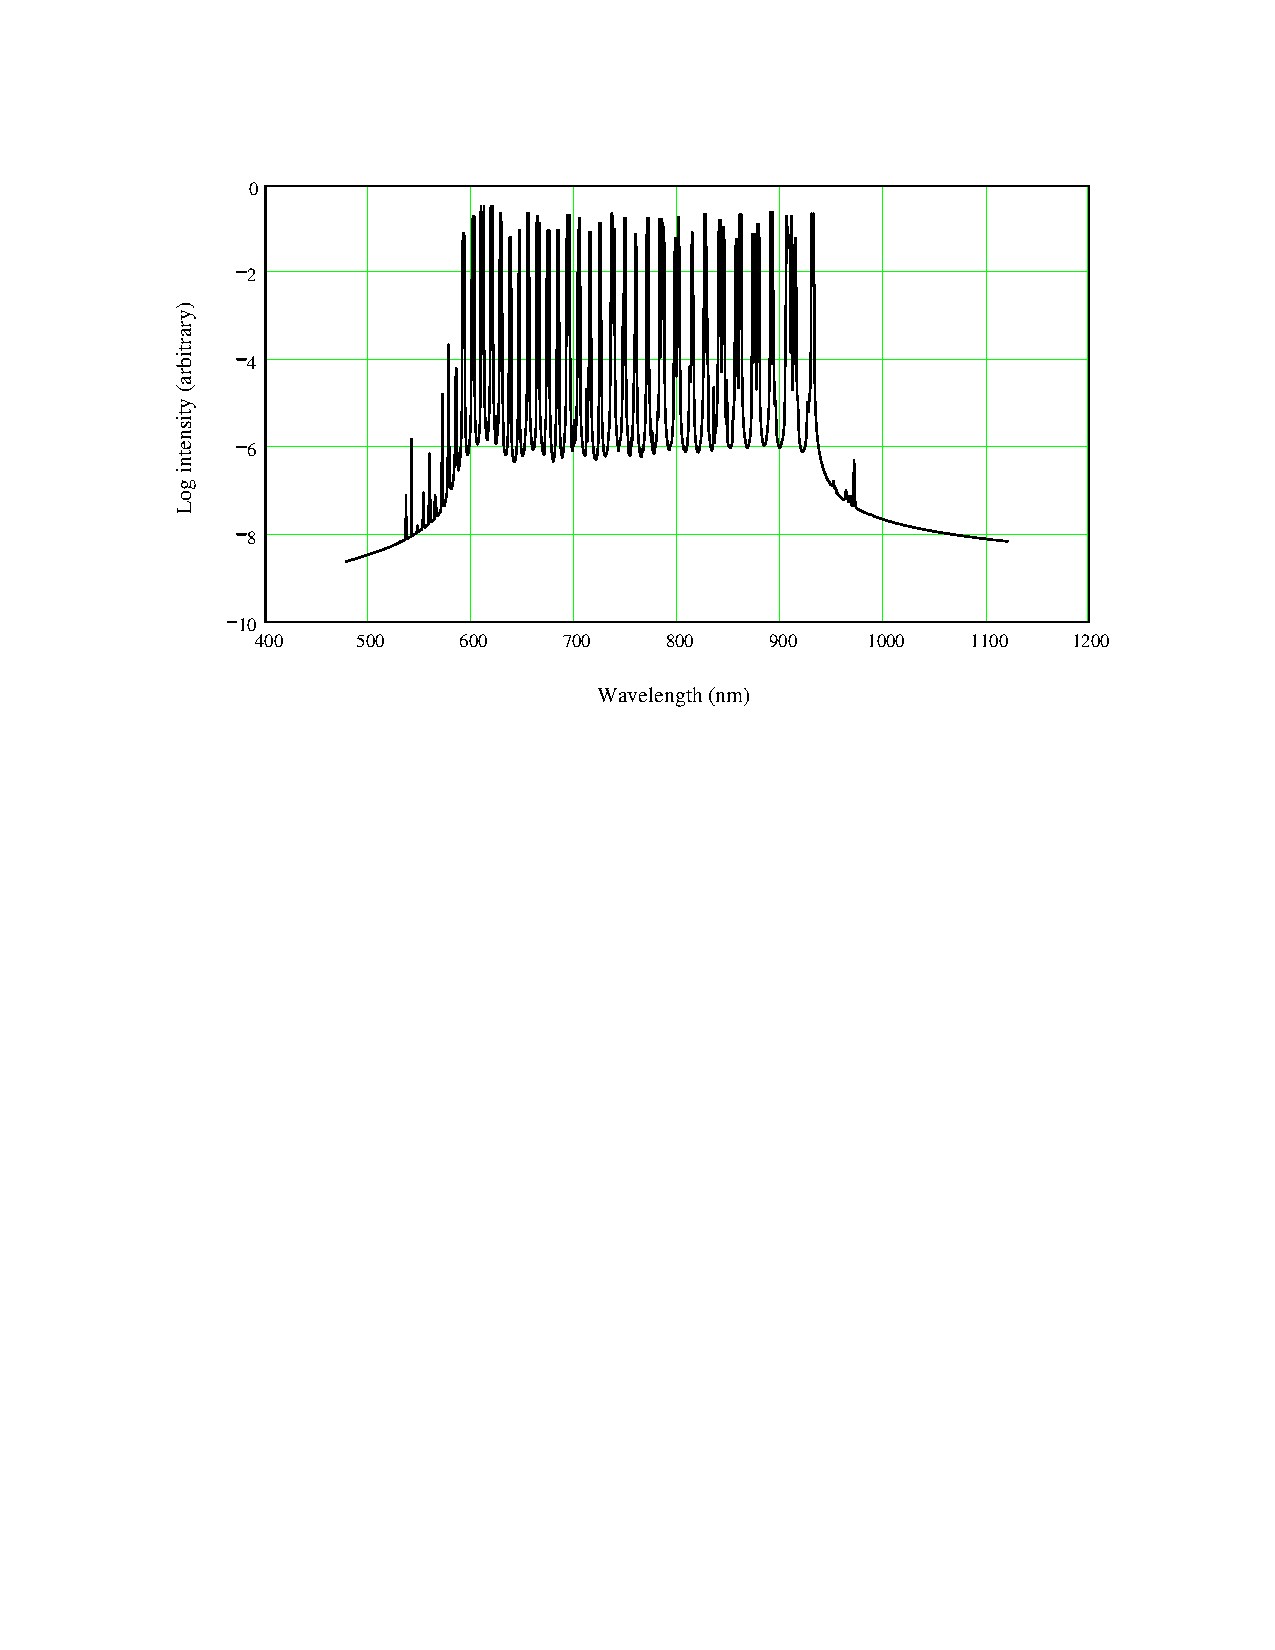
\includegraphics[bb=50 450 489 680]
{non-target_1/non-target_1.pdf}
}
\caption[Simulated single color LIF from non-target molecule (iodine non-isotope)]{Simulated single color LIF from non-target molecule (iodine non-isotope)}
\label{non-target_1}
\end{figure}
%----------------------------------------------------------------------------

%----------------------------------------------------------------------------
%----------------------------------------------------------------------------
From these final upper state distributions a fluorescence spectrum is calculated. Each energy level in the calculated upper B state distribution is connected, in a $J=\pm1$ pair, to each X vibrational state. A ``fluorescence line strength'', $S$, is assigned to each possible downward transition and approximated by
%----------------------------------------------------------------------------
\begin{equation}
S(\nu^{\prime\prime},\nu^{\prime})
=
P^{\prime}FCF(\nu^{\prime\prime},\nu^{\prime})
\end{equation}
%----------------------------------------------------------------------------
%----------------------------------------------------------------------------
%----------------------------------------------------------------------------
%bb defines the bounding box for the pdf
%viewport defines the area of the pdf used
%in sidewaysfigure the last entry in bb moves the caption toward/away the pic
%in sidewaysfigure the second entry in bb moves the pic toward/away the caption
%----------------------------------------------------------------------------
\begin{figure}
\scalebox{0.8}[0.8]{
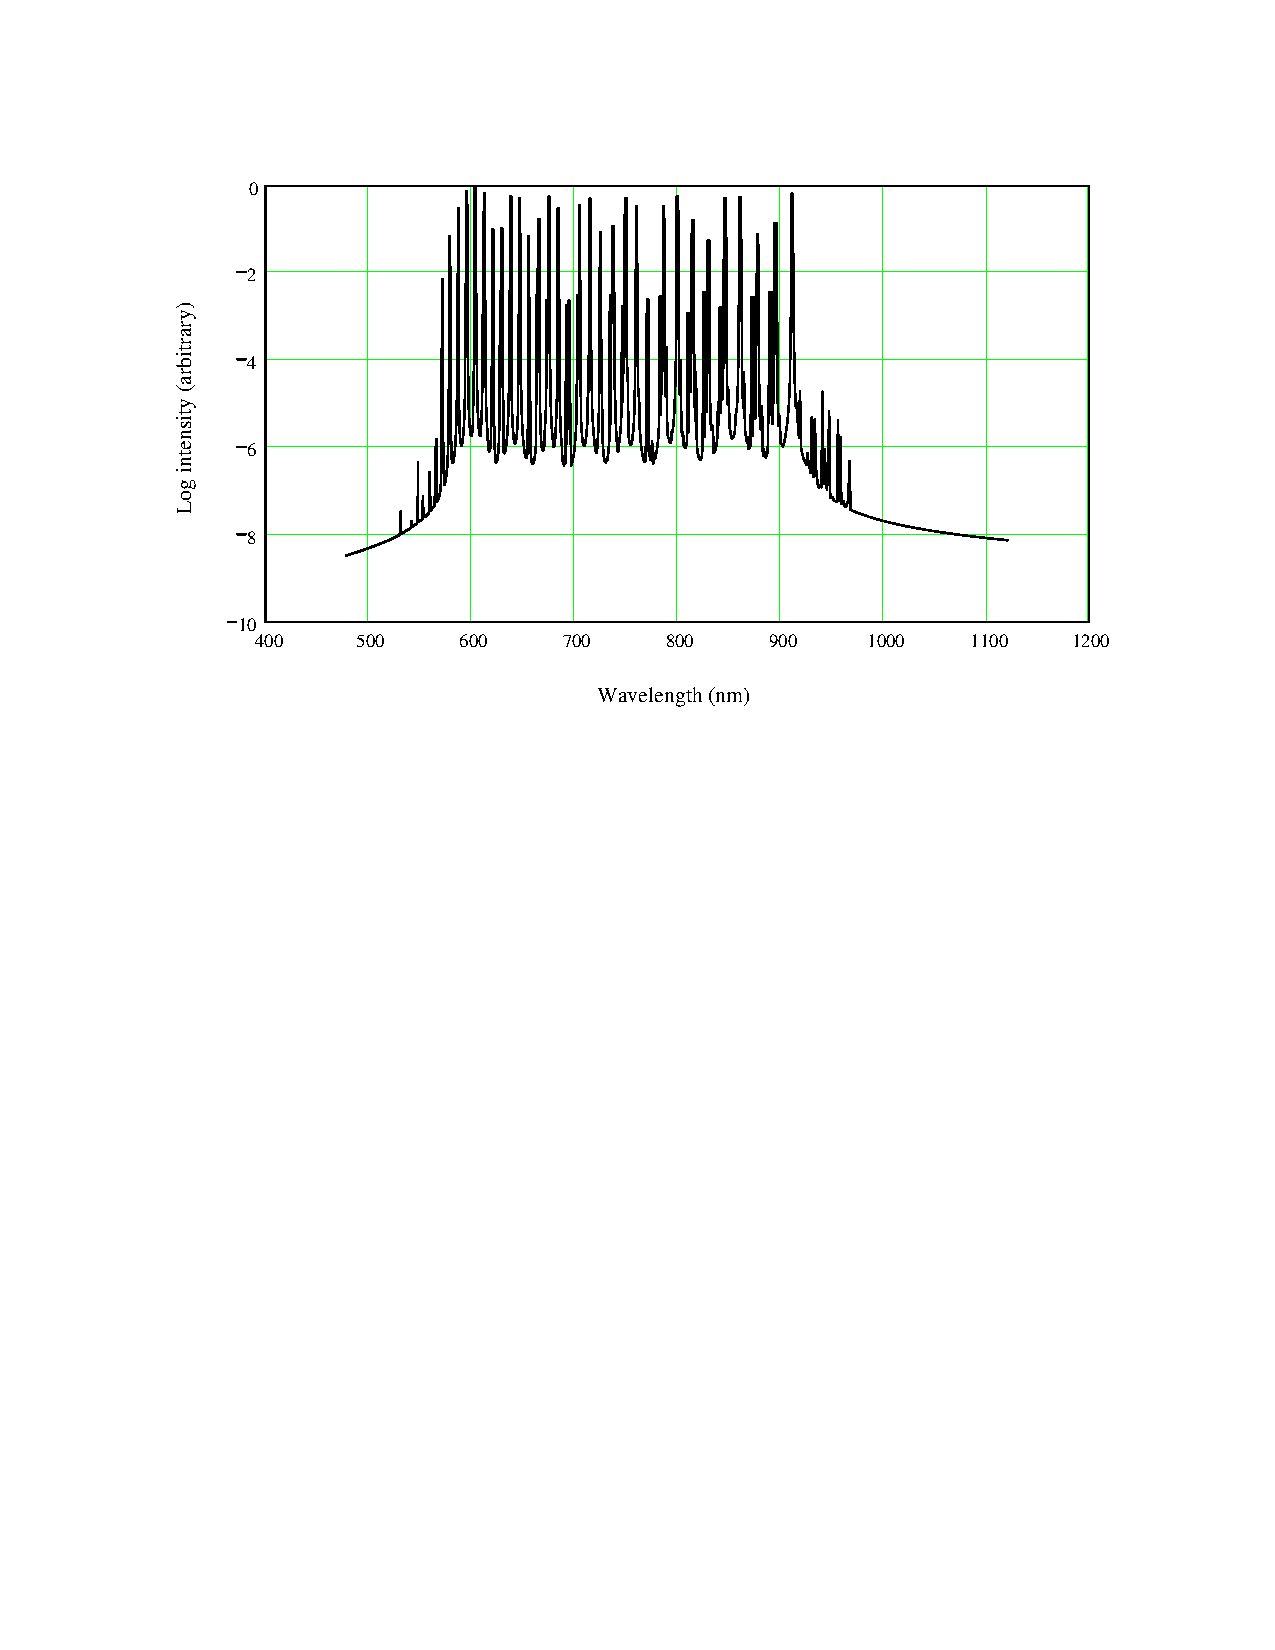
\includegraphics[bb=50 450 489 680]
{target_1/target_1.pdf}
}
\caption[Simulated single color LIF from target molecule (iodine isotope)]{Simulated single color LIF from target molecule (iodine isotope)}
\label{target_1}
\end{figure}
%----------------------------------------------------------------------------

%----------------------------------------------------------------------------
where $P^{\prime}$ is the initial population of the fluoresceing B level ($\nu^{\prime\prime}$) calculated for each pathway, and $\nu^{\prime}$ is the vibrational number of the lower X vibrational level. The resulting fluorescence signal from each transition is modeled by Equation \ref{lorentzian} by assigning each J-split pair to a Lorentzian scaled by $S$. See Figure \ref{non-target_1}, \ref{target_1}, and \ref{target_3} for a plots of the resulting signal from summing the transitions for a few basic pathways. Note that when one considers the result from Section \ref{side} (only around one thousand of iodine molecules emit into the detector in the benchtop geometry) we see that verification of these high extinction ratios becomes unlikely unless we move to a LIDAR type geometry.
%----------------------------------------------------------------------------
%----------------------------------------------------------------------------
%bb defines the bounding box for the pdf
%viewport defines the area of the pdf used
%in sidewaysfigure the last entry in bb moves the caption toward/away the pic
%in sidewaysfigure the second entry in bb moves the pic toward/away the caption
%----------------------------------------------------------------------------
\begin{figure}
\scalebox{0.8}[0.8]{
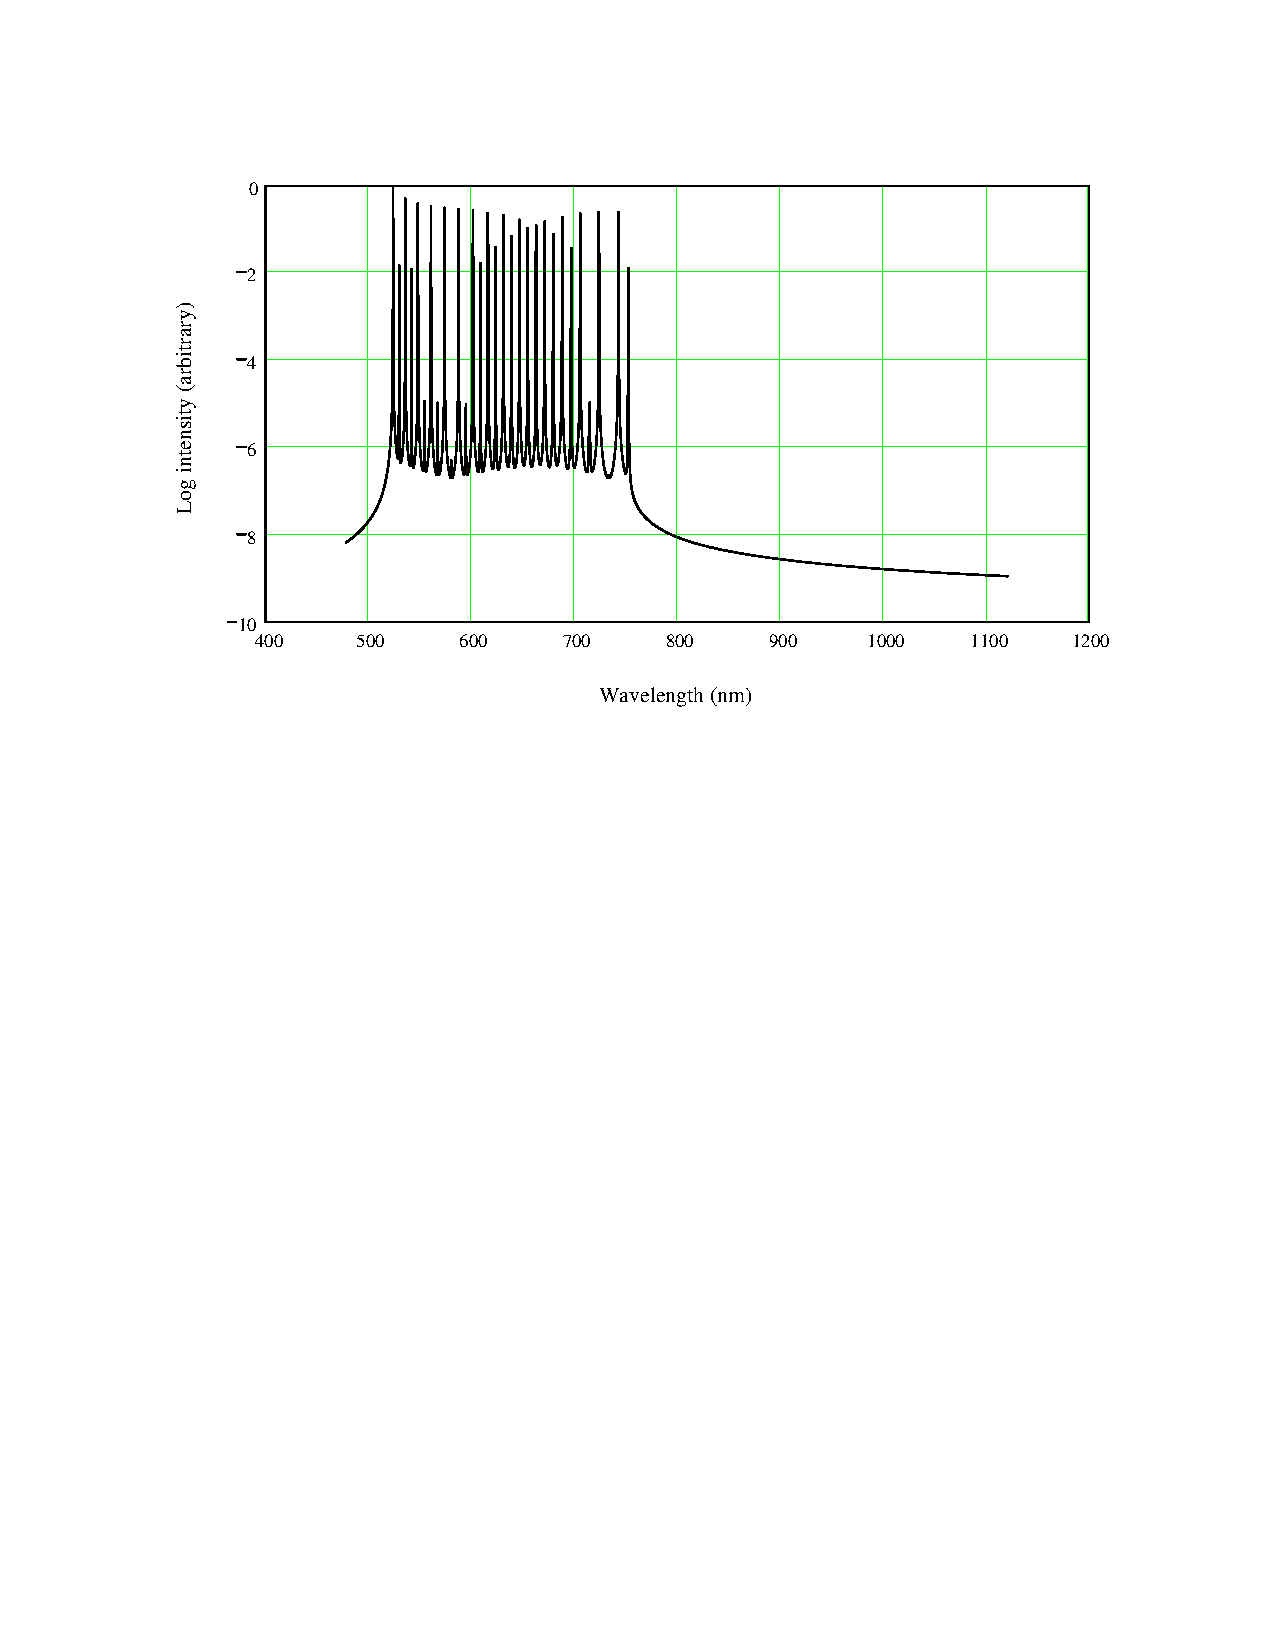
\includegraphics[bb=50 450 489 680]
{target_3/target_3.pdf}
}
\caption[Simulated three color LIF from target molecule (iodine isotope)]{Simulated three color LIF from target molecule (iodine isotope). These simulations show that the three color LIF (shown here) is around 8 orders of magnitude more intense than the single color responce of the target and non-target (see Figures \ref{target_1} and \ref{non-target_1}) in the spectral region near 520 nm.}
\label{target_3}
\end{figure}
%----------------------------------------------------------------------------

%----------------------------------------------------------------------------
%----------------------------------------------------------------------------
%----------------------------------------------------------------------------
%----------------------------------------------------------------------------
%----------------------------------------------------------------------------
%----------------------------------------------------------------------------
%----------------------------------------------------------------------------
